\chapter{Communication interfaces}
All the communication interfaces are available via dedicated connectors.

\begin{ZubaxTableWrapper}{Connectors types}
    \begin{ZubaxWrappedTable}{| X | X |}
    Connector name          & Connector type    \\
    CAN1 (2 connectors)     & JST BM04B-GHS     \\
    CAN2 (2 connectors)     & JST BM04B-GHS     \\
    AUX                     & JST BM04B-GHS     \\
    USB                     & USB 2.0 Micro-B   \\
\end{ZubaxWrappedTable}
\end{ZubaxTableWrapper}


\begin{figure}[!hbt]
    \centering
    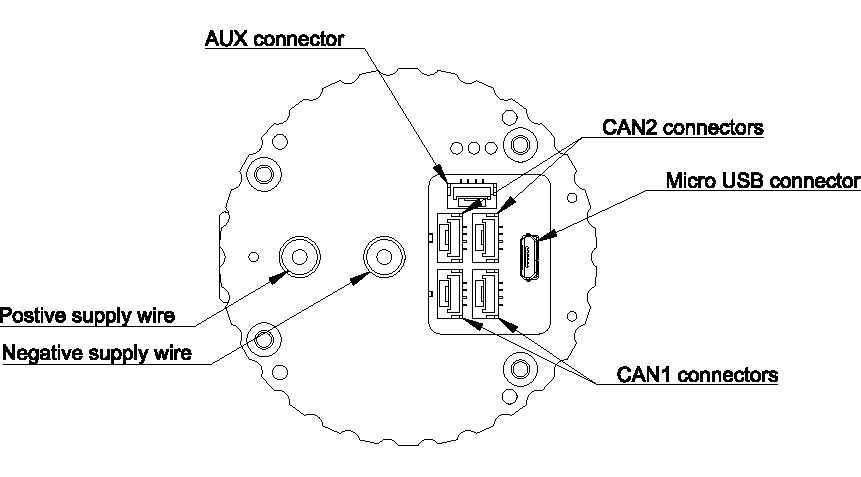
\includegraphics[width=1\textwidth]{figures/connectors_placement.pdf}
    \caption{Connectors drawing}
\end{figure}

\begin{figure}[!hbt]
    \centering
    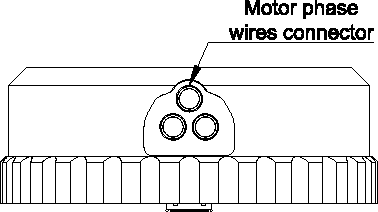
\includegraphics[width=0.5\textwidth]{figures/phase_wires.pdf}
    \caption{Motor phase wires connector drawing}
\end{figure}

\newpage

\section{CAN bus}
The device is equipped with a doubly redundant ISO 11898-2 CAN 2.0A/B interface.
Each CAN interface has two standard UAVCAN Micro connectors\footnote{Refer to \url{http://uavcan.org}
for more information on UAVCAN.} that are joined in parallel. Note that the device does not 
terminate the CAN bus internally.

The secondary CAN bus interface (CAN2) can only be used with redundant CAN bus configurations.
With non-redundant CAN bus configurations, only the primary CAN bus connectors (CAN1) can be used; the secondary
CAN2 bus connectors should be left empty.

\begin{ZubaxSimpleTable}{CAN bus connectors pinout}{|c X X X[3]|}
	Pin no. & Type         & Name      & Comment \\
	1       & Power        & PWR       & Not connected to the device's circuits internally.\\
	2       & Input/Output & CAN H     & \\
	3       & Input/Output & CAN L     & \\
	4       & Ground       & GND       & \\
\end{ZubaxSimpleTable}

\subsection{BEC output}
Zubax Komar features one software-controllable BEC output per CAN interface which can be accessed using the
bus power supply pins on the UAVCAN connectors. The BEC outputs are protected against short-circuits to
a maximum output current of 500\,mA per CAN interface. The outputs are also protected from reverse current
flows with ideal diodes. BEC outputs for both CAN interfaces are controlled by a single software parameter.

\section{USB interface}
Komar features a full-speed USB 2.0 port with a standard CDC ACM interface providing driverless compatibility
with all major operating systems (GNU/Linux, Windows, Mac OS X). It is sometimes termed the
\emph{virtual serial port}. It accepts a standard USB Micro-B connector and will report the
following properties to the USB host when connected:
\begin{itemize}
    \item Vendor ID -- 0x1D50
    \item Product ID -- 0x60C7
    \item Vendor string -- Zubax Robotics 
    \item Device description string -- Zubax Robotics Telega
\end{itemize}
The USB interface uses Popcop protocol to communicate with Kucher, the GUI software for \text{T\'elega}-based
products.

\section{GPIO}
Zubax Komar is equipped with two GPIO pins that are available on the AUX connector. While GPIO2 can only be used
for GPIO purposes, GPIO1 permits additional functions to be enabled using software. These functions are: 1) the
thermistor input; and 2) the RC PWM input.

\begin{ZubaxSimpleTable}{AUX connector pinout}{|c X X X[3]|}
	Pin no. & Type         & Name      & Comment                          \\
	1       & Power        & PWR       & 5\,V power line output           \\
	2       & Input/Output & GPIO1     & RC PWM input or Thermistor input \\
	3       & Input/Output & GPIO2     &                                  \\
	4       & Ground       & GND       &                                  \\
\end{ZubaxSimpleTable}

\subsection{Thermistor input}
The PTC thermistor measures the motor windings temperature. Komar supports KTY84/130, KTY81/120 and KTY83/120
thermistors and no additional components are needed to connect the thermistor. The thermistor model can be
configured in the firmware. The thermistor should be connected between the GPIO1 and GROUND pins of the AUX
connector.

Note that most commercially-available BLDC motors do not have an embedded temperature sensor and therefore
require the end-user to install one. This is a relatively simple procedure that involves: 1) soldering
extension wires to the thermistor; and 2) gluing the thermistor to the motor winding with epoxy resin.

\subsection{RC PWM input}
Zubax Komar also supports the older analog RC PWM interface. Although this may be slow and prone
to electromagnetic interference, it remains one of the most widely-used ESC interfaces in the industry.

The RC PWM input should be connected to the GPIO1 of the AUX connector and then configured in the firmware.
\text{T\'elega} firmware is highly configurable when using the RC PWM interface. For a detailed description,
please refer to the \text{T\'elega} reference manual.
